\documentclass[12pt]{article}
\usepackage[left=1cm, right=1cm, top=2cm,bottom=1.5cm]{geometry} 

\usepackage[parfill]{parskip}
\usepackage[utf8]{inputenc}
\usepackage[T2A]{fontenc}
\usepackage[russian]{babel}
\usepackage{enumitem}
\usepackage[normalem]{ulem}
\usepackage{amsfonts, amsmath, amsthm, amssymb, mathtools,xcolor,accents}
\usepackage{blkarray}

\usepackage{tabularx}
\usepackage{hhline}

\usepackage{accents}
\usepackage{fancyhdr}
\pagestyle{fancy}
\renewcommand{\headrulewidth}{1.5pt}
\renewcommand{\footrulewidth}{1pt}

\usepackage{graphicx}
\usepackage[figurename=Рис.]{caption}
\usepackage{subcaption}
\usepackage{float}

%%Наименование папки откуда забирать изображения
\graphicspath{ {./images/} }

%%Изменение формата для ввода доказательства
\renewcommand{\proofname}{$\square$  \nopunct}
\renewcommand\qedsymbol{$\blacksquare$}

%%Изменение отступа на таблицах
\addto\captionsrussian{%
	\renewcommand{\proofname}{$\square$ \nopunct}%
}
%% Римские цифры
\newcommand{\RN}[1]{%
	\textup{\uppercase\expandafter{\romannumeral#1}}%
}

%% Для удобства записи
\newcommand{\MR}{\mathbb{R}}
\newcommand{\MC}{\mathbb{C}}
\newcommand{\MQ}{\mathbb{Q}}
\newcommand{\MN}{\mathbb{N}}
\newcommand{\MZ}{\mathbb{Z}}
\newcommand{\MBE}{\mathbb{E}}
\newcommand{\MTB}{\mathbb{T}}
\newcommand{\MTI}{\mathbb{I}}
\newcommand{\MI}{\mathrm{I}}
\newcommand{\MCI}{\mathcal{I}}
\newcommand{\MCR}{\mathcal{R}}
\newcommand{\MJ}{\mathrm{J}}
\newcommand{\MH}{\mathrm{H}}
\newcommand{\MT}{\mathrm{T}}
\newcommand{\MU}{\mathcal{U}}
\newcommand{\MV}{\mathcal{V}}
\newcommand{\MA}{\mathcal{A}}
\newcommand{\MB}{\mathcal{B}}
\newcommand{\MF}{\mathcal{F}}
\newcommand{\ME}{\mathcal{E}}
\newcommand{\MW}{\mathcal{W}}
\newcommand{\ML}{\mathcal{L}}
\newcommand{\MM}{\mathcal{M}}
\newcommand{\MP}{\mathcal{P}}
\newcommand{\VN}{\varnothing}
\newcommand{\VE}{\varepsilon}
\newcommand{\dx}{\, dx}
\newcommand{\dy}{\, dy}
\newcommand{\dz}{\, dz}
\newcommand{\dd}{\, d}


\theoremstyle{definition}
\newtheorem{defn}{Опр:}
\newtheorem{rem}{Rm:}
\newtheorem{prop}{Утв.}
\newtheorem{exrc}{Упр.}
\newtheorem{problem}{Задача}
\newtheorem{lemma}{Лемма}
\newtheorem{theorem}{Теорема}
\newtheorem{corollary}{Следствие}

\newenvironment{cusdefn}[1]
{\renewcommand\thedefn{#1}\defn}
{\enddefn}

\DeclareRobustCommand{\divby}{%
	\mathrel{\text{\vbox{\baselineskip.65ex\lineskiplimit0pt\hbox{.}\hbox{.}\hbox{.}}}}%
}
\DeclareRobustCommand{\ndivby}{\mkern-1mu\not\mathrel{\mkern4.5mu\divby}\mkern1mu}


%Короткий минус
\DeclareMathSymbol{\SMN}{\mathbin}{AMSa}{"39}
%Длинная шапка
\newcommand{\overbar}[1]{\mkern 1.5mu\overline{\mkern-1.5mu#1\mkern-1.5mu}\mkern 1.5mu}
%Функция знака
\DeclareMathOperator{\sgn}{sgn}

%Функция ранга
\DeclareMathOperator{\rk}{\text{rk}}
\DeclareMathOperator{\diam}{\text{diam}}


%Обозначение константы
\DeclareMathOperator{\const}{\text{const}}
\DeclareMathOperator{\id}{\text{id}}
\DeclareMathOperator{\codim}{\text{codim}}

\DeclareMathOperator*{\dsum}{\displaystyle\sum}
\newcommand{\ddsum}[2]{\displaystyle\sum\limits_{#1}^{#2}}
\newcommand{\ddssum}[2]{\displaystyle\smashoperator{\sum\limits_{#1}^{#2}}}
\newcommand{\ddlsum}[2]{\displaystyle\smashoperator[l]{\sum\limits_{#1}^{#2}}}
\newcommand{\ddrsum}[2]{\displaystyle\smashoperator[r]{\sum\limits_{#1}^{#2}}}

%Интеграл в большом формате
\DeclareMathOperator{\dint}{\displaystyle\int}
\newcommand{\ddint}[2]{\displaystyle\int\limits_{#1}^{#2}}
\newcommand{\ssum}[1]{\displaystyle \sum\limits_{n=1}^{\infty}{#1}_n}

\newcommand{\smallerrel}[1]{\mathrel{\mathpalette\smallerrelaux{#1}}}
\newcommand{\smallerrelaux}[2]{\raisebox{.1ex}{\scalebox{.75}{$#1#2$}}}

\newcommand{\smallin}{\smallerrel{\in}}
\newcommand{\smallnotin}{\smallerrel{\notin}}

\newcommand*{\medcap}{\mathbin{\scalebox{1.25}{\ensuremath{\cap}}}}%
\newcommand*{\medcup}{\mathbin{\scalebox{1.25}{\ensuremath{\cup}}}}%

\makeatletter
\newcommand{\vast}{\bBigg@{3.5}}
\newcommand{\Vast}{\bBigg@{5}}
\makeatother

%Промежуточное значение для sup\inf, поскольку они имеют разную высоту
\newcommand{\newsup}{\mathop{\smash{\mathrm{sup}}}}
\newcommand{\newinf}{\mathop{\mathrm{inf}\vphantom{\mathrm{sup}}}}

%Скалярное произведение
\newcommand{\inner}[2]{\left\langle #1, #2 \right\rangle }
\newcommand{\linsp}[1]{\left\langle #1 \right\rangle }
\newcommand{\linmer}[2]{\left\langle #1 \vert #2\right\rangle }

%Подпись символов снизу
\newcommand{\ubar}[1]{\underaccent{\bar}{#1}}

%%Шапка для букв сверху
\newcommand{\wte}[1]{\widetilde{#1}}
\newcommand{\wht}[1]{\widehat{#1}}
\newcommand{\ovl}[1]{\overline{#1}}
\newcommand{\unl}[1]{\underline{#1}}


%%Трансформация Фурье
\newcommand{\fourt}[1]{\mathcal{F}\left(#1\right)}
\newcommand{\ifourt}[1]{\mathcal{F}^{-1}\left(#1\right)}

%%Символ вектора
\newcommand{\vecm}[1]{\overrightarrow{#1\,}}

%%Пространстов матриц
\newcommand{\matsq}[1]{\operatorname{Mat}_{#1}}
\newcommand{\mat}[2]{\operatorname{Mat}_{#1, #2}}

%Оператор для действ и мнимых чисел
\DeclareMathOperator{\IM}{\operatorname{Im}}
\DeclareMathOperator{\RE}{\operatorname{Re}}
\DeclareMathOperator{\li}{\operatorname{li}}
\DeclareMathOperator{\GL}{\operatorname{GL}}
\DeclareMathOperator{\SL}{\operatorname{SL}}
\DeclareMathOperator{\Char}{\operatorname{char}}
\DeclareMathOperator\Arg{Arg}
\DeclareMathOperator\ord{ord}

%Оператор для образа
\DeclareMathOperator{\Ima}{Im}

%Делимость чисел
\newcommand{\modn}[3]{#1 \equiv #2 \; (\bmod \; #3)}
\newcommand{\nmodn}[3]{#1 \not\equiv #2 \; (\bmod \; #3)}

%%Взятие в скобки, модули и норму
\newcommand{\parfit}[1]{\left( #1 \right)}
\newcommand{\modfit}[1]{\left| #1 \right|}
\newcommand{\sqparfit}[1]{\left\{ #1 \right\}}
\newcommand{\normfit}[1]{\left\| #1 \right\|}

%%Функция для обозначения равномерной сходимости по множеству
\newcommand{\uconv}[1]{\overset{#1}{\rightrightarrows}}
\newcommand{\uconvm}[2]{\overset{#1}{\underset{#2}{\rightrightarrows}}}

%% Функция для добавления круга сверху множества
\newcommand{\Circ}[1]{\accentset{\circ}{#1}}

%% Жирное подчеркивание
\newcommand{\buline}[1]{\textbf{\uline{#1}}}

%%Функция для обозначения нижнего и верхнего интегралов
\def\upint{\mathchoice%
	{\mkern13mu\overline{\vphantom{\intop}\mkern7mu}\mkern-20mu}%
	{\mkern7mu\overline{\vphantom{\intop}\mkern7mu}\mkern-14mu}%
	{\mkern7mu\overline{\vphantom{\intop}\mkern7mu}\mkern-14mu}%
	{\mkern7mu\overline{\vphantom{\intop}\mkern7mu}\mkern-14mu}%
	\int}
\def\lowint{\mkern3mu\underline{\vphantom{\intop}\mkern7mu}\mkern-10mu\int}

%%След матрицы
\DeclareMathOperator*{\tr}{tr}

\DeclareMathOperator*{\symdif}{\bigtriangleup}

% Верхние\нижние пределы
\DeclareMathOperator*\lowlim{\underline{lim}}
\DeclareMathOperator*\uplim{\overline{lim}}

\makeatletter
\renewcommand*\env@matrix[1][*\c@MaxMatrixCols c]{%
	\hskip -\arraycolsep
	\let\@ifnextchar\new@ifnextchar
	\array{#1}}
\makeatother


%% Переопределение функции хи, чтобы выглядела более приятно
\makeatletter
\@ifdefinable\@latex@chi{\let\@latex@chi\chi}
\renewcommand*\chi{{\@latex@chi\smash[t]{\mathstrut}}} % want only bottom half of \mathstrut
\makeatletter

\setcounter{MaxMatrixCols}{20}

\begin{document}
\lhead{Классическая дифф. геометрия}
\chead{Пенской А.В.}
\rhead{Лекция - 1}
\section*{Введение}
\uline{\textbf{Цель курса}}: понять на простых объектах что такое кривизна, в чём её смысл, как её можно описать, измерить и что с ней можно делать в математическом смысле? 

``Классическая'' в нашем случае означает, что мы будем рассматривать только объекты дифференциальной геометрии $\RN{19}$-го века, а именно кривые и поверхности (возможно в многомерном пространстве) в Евклидовом пространстве. 

Дифференциальная геометрия гладких многообразий и расслоений изучается в следующем курсе дифференциальной геометрии и топологии.

\subsection*{Гладкие регулярные параметризованные кривые}
Начнём с рассмотрения вопроса того, что такое кривая. Из аналитической геометрии мы помним кривые второго порядка, которые задаются многочленом второй степени в виде: $F(x,y) = 0$. Были геометрические места точек, чьи координаты удовлетворяют этому уравнению (точки, заданные этим уравнением), но на самом деле мы работали с некоторыми классами эквивалентности уравнений. 

Таким образом, связь между г.м.т. и уравнением уже не очень прямое. Например, были разные квадрики, которые задавали одно и тоже множество: пустое множество могло быть множеством точек разных мнимых эллипсов. 

В дифференциальной геометрии мы начнем с гладкой кривой. Интуитивно, гладкой кривой мы можем назвать график гладкой функции - то, что естественно приходит на ум.

\begin{figure}[H]
	\centering
	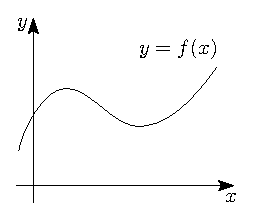
\includegraphics[width=0.25\textwidth]{CDGL1_1.eps}
	\caption{График гладкой кривой.}
	\label{1_1}
\end{figure}
Степень гладкости может быть разной, нам это пока не важно. Зато заметим, что у нас есть два разных способа описания кривых:
\begin{enumerate}[label=\arabic*)]
	\item \uwave{Неявное описание кривой}: $F(x,y) = 0$ (аналитическая геометрия);
	\item \uwave{Параметрическое описание кривой}: $x = x(t), \, y = y(t)$ (физика, механика, ан. геометрия);
\end{enumerate}
\textbf{Неявное описание кривой} обычно рассматривали на аналитической геометрии, где соотношение задает некоторое множество точек. Как мы уже видели, там всё не совсем очевидно с точки зрения гладкости кривых и функций.

\textbf{Пример}: $F(x,y) = xy = 0$ - гладкая функция, как по $x$, так и по $y$, но это координатный крест и его вряд ли можно назвать гладкой кривой, поскольку есть особая точка в $0$.
\begin{figure}[H]
	\centering
	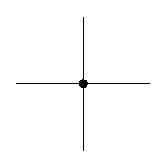
\includegraphics[width=0.1\textwidth]{CDGL1_2.eps}
	\caption{Крест: $F(x,y) = xy = 0$.}
	\label{1_2}
\end{figure}
\textbf{Параметрическое описание кривой} означает, что координаты заданы как функции от некоторой новой перменной, которая называется параметром. В данном случае наша кривая представляет собой траекторию движения некоторого тела или частицы. 
\begin{figure}[H]
	\centering
	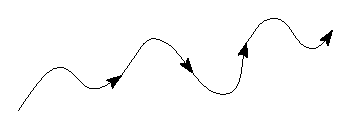
\includegraphics[width=0.2\textwidth]{CDGL1_3.eps}
	\caption{Траектория движения.}
	\label{1_3}
\end{figure}

Аналогично с параметризация мы сталкивались в аналитической геометрии, поскольку для кривых второго порядка можно написать тригонометрическую параметризацию.

\textbf{Пример}: $x = \cos{t}, \, y = \sin{t}$ - параметрическое описание окружности радиуса $1$.
\begin{figure}[H]
	\centering
	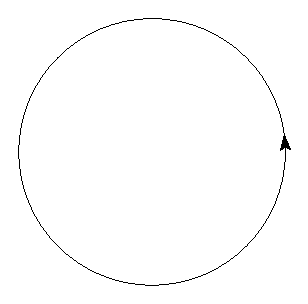
\includegraphics[width=0.1\textwidth]{CDGL1_4.eps}
	\caption{Тригонометрическая параметризация.}
	\label{1_4}
\end{figure}

Часто в курсе аналитической геометрии доказывают факт, что если имеется квадрика (пусть она не особая), то мы можем взять на ней некоторую точку $O$ и некоторую прямую вне квадрики, тогда есть соответствие: проводя прямую через точку $O$ каждой точке $A$ на нашей квадрике отвечает точка $A'$ на выбранной прямой.
\begin{figure}[H]
	\centering
	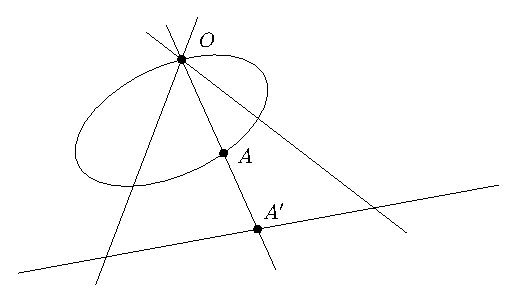
\includegraphics[width=0.4\textwidth]{CDGL1_5.eps}
	\caption{Параметризация квадрики на прямой.}
	\label{1_5}
\end{figure} 
Если мы на этой прямой введём некоторую параметризацию, тогда мы сможем вычислить координаты точек на квадрике:
$$
	A' = (a + bt, c + dt) \Rightarrow A = \left(\tfrac{P(t)}{Q(t)},\tfrac{R(t)}{S(t)}\right)
$$
где координаты точки $A$ будут состоять из рациональных функций на $t$, которые будут иметь степень не выше $2$. Это получится так называемая рациональная параметризация квадрики.

Какой из этих способов параметризации нам будет интереснее? В алгебраической геометрии интереснее неявное задание, тогда как нам будет интереснее и естественнее параметрическое задание. Тем не менее, даже в таком подходе нас ожидает ряд тонкостей: даже если $x(t), y(t)$ гладкие, то можно создать гладкую кривую (в смысле гладкости координат), которая будет устроена как ``уголок''.
\begin{figure}[H]
	\centering
	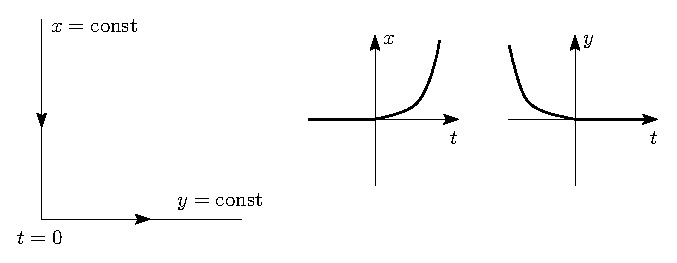
\includegraphics[width=0.6\textwidth]{CDGL1_6.eps}
	\caption{Гладкая по параметрам функция.}
	\label{1_6}
\end{figure}
С помощью экспоненты достаточно легко построить такую функцию. Таким образом, нужно понять что плохого происходит в точке $t = 0$ и почему условий гладкости нам недостаточно. Рассмотрим, что происходит в такой функции с производными: 
\begin{enumerate}[label=\arabic*)]
	\item $t < 0 \Rightarrow x(t) = \const \Rightarrow x'(t) = 0 \Rightarrow$ по непрерывности в $t = 0, \, x'(t) = 0$;
	\item $t > 0 \Rightarrow y(t) = \const \Rightarrow y'(t) = 0 \Rightarrow$ по непрерывности в $t = 0, \, y'(t) = 0$;
\end{enumerate}
В результате: $t = 0 \Rightarrow x' = 0,\, y' = 0$. Если мы считаем, что наша кривая это радиус-вектор: 
$$
	\vec{r}(t) = (x(t), y(t)) \Rightarrow \dfrac{d\vec{r}}{dt}(t) = (x'(t), y'(t))
$$
где $\tfrac{d\vec{r}}{dt}(t)$ - вектор скорости, то в $t = 0$ скорость обращается в $0$, поэтому мы будем требовать, чтобы таких точек не было.

\begin{defn}
	\uwave{Гладкая регулярная параметризованная кривая} (ГРП) в $\MR^n$ - это отображение: 
	$$
		\vec{r} = r \colon (a,b) \to \MR^n, \; (a,b)\subset \MR
	$$ 
	причём $\vec{r}(t) = (x^1(t), \dotsc, x^n(t))$ - набор координатных функций, где все $x^i(t)$ - гладкие и выполнено условие регулярности:
	$$
		\forall t\in (a,b), \, \dfrac{d \vec{r}}{dt}(t) = (\dot{x}^1(t), \dotsc, \dot{x}^n(t)) \neq 0
	$$
\end{defn}

\begin{rem}
	Евклидову систему координат мы будем отождествлять с $\MR^n$. 
\end{rem}
\begin{rem}
	Под гладкостью мы будем понимать либо класс функций $C^\infty$, либо $C^k$, где $k$ - велико, поскольку в геометрии не придается много значению именно этому параметру. Если кривая будет трижды дифференцируема $(C^3)$, то все теоремы будут работать.
\end{rem}

Для чего нужно условие регулярности? Пусть у нас есть значение параметра $t_0$ и $\tfrac{d\vec{r}}{dt}(t_0) \neq 0$, значит $\exists \, i \colon \dot{x}^i(t_0) \neq 0 \Rightarrow$ по теореме об обратной функции $\exists \, t = t(x^i)$ в некоторой окрестности $x^i(t_0)$. Следовательно, это можно подставить в исходное уравнение:
$$
	\vec{r} = (x^1(t(x^i)), \dotsc, x^n(t(x^i)))	
$$
Таким образом, условие регулярности гарантирует, что мы можем заменить параметр и кривая параметризованная будет устроена как, например, график гладкой функции для двух переменных. 

\textbf{Пример}: Если $n = 2$, то такой процедурой мы получим $(x, y(x))$ - график гладкой функции.

В случае многих переменных, мы получим некоторый аналог, когда все переменные, кроме какой-то выделенной, будут гладкими функциями от выделенной переменной, поскольку обратная функция будет гладкой и композиция гладких функций также будет гладкой. В результате, в заданных условиях ``уголков'' у нас не будет.

\subsection*{Перепараметризация кривой}
Пусть у нас задана ГРП кривая $\vec{r}(t)$. Предположим, что $t = \varphi(\tau)$, тогда получим: $\vec{r}(\varphi(\tau))$, где: 
$$
	\varphi \colon (a,b) \to (a',b') \Rightarrow \vec{r}(\varphi(\tau))\colon (a',b') \to \MR^n
$$ 
Формально говоря, у нас будет некоторая новая гладкая кривая, но как ГМТ (геом. место точек) это будет тем же самым. Обычно заменяют параметры без дополнительных пояснений. 
\begin{defn}
	\uwave{Перепараметризацией} или \uwave{репараметризацией} кривой $\vec{r}(t)$ называется замена параметра $t$ на $\varphi(\tau)$ в гладкой регулярной параметризованной кривой.
\end{defn}

\begin{rem}
	Не всякая замена делает из регулярной кривой - регулярную кривую.
\end{rem}

\begin{prop}
	Если $\vec{r}(t)$ - ГРП, $\varphi(\tau)$ - репараметризация и $\varphi'(\tau) \neq 0$, то $\vec{r}(\varphi(\tau))$ - тоже регулярная кривая.
\end{prop}
\begin{proof}
	Посчитаем производную:
	$$
		\dfrac{d}{d\tau}\vec{r}(\varphi(\tau)) = \underbrace{\dfrac{d\vec{r}}{d t}(\varphi(\tau))}_{\neq 0}{\cdot}\varphi'(\tau)
	$$
	Следовательно, чтобы новая кривая была регулярной нужно, чтобы $\varphi'(\tau) \neq 0$.
\end{proof}

Мы рисуем стрелочки на рисунках, поскольку они означают \uline{ориентацию кривой}.
\begin{defn}
	\uwave{Ориентацией кривой} называется направление в котором мы двигаемся, когда параметр возрастает.
\end{defn}
Что происходит при перепараметризации? 
\begin{enumerate}[label=\arabic*)]
	\item Если $\varphi'(\tau) > 0$, то ориентация не изменится;
	\item Если $\varphi'(\tau) < 0$, то ориентация изменится на противоположную;
\end{enumerate}

\begin{rem}
	Если есть две кривые, одна из которых является перепараметризацией другой, то они определяют одно и тоже ГМТ, поэтому иногда в некоторых книгах кривой называют класс эквивалентности параметризованных кривых, где две кривые эквивалентны, если одна из них это перепараметризация другой $\Rightarrow$ легко понять, что перепараметризация это отношение эквивалентности на множестве кривых.
	
	Какого-то одного подхода, который был бы явно лучше - нет. Мы будем придерживаться подхода, что перепараметризованные кривые - разные, но при этом мы будем понимать, что ГМТ у них общее. Данное соглашение принято в почти всех современных книгах.
\end{rem}
\newpage

\section*{Пример обозначений ГРП кривой}

\textbf{\uline{Обозначение}}: Мы будем придерживаться следующих обозначений: $\vec{r}(\varphi(\tau)) = \vec{r}(\tau)$.

Пусть $\MBE^2$ - евклидова плоскость - просто аффинное пространство, в котором есть скалярное произведение и ничего больше. Пусть $O \in \MBE^2$, определим отображение:
$$
	f \colon \MBE^2 \to \MR, \, f(P) = \left|\vecm{OP}\right|
$$
Заметим, что это геометрическое определение $\Rightarrow$ здесь нет координат, базисных векторов. Есть только аффинное пространство. $f$ - для каждой точки определяет расстояние от $O$ до неё. Введём теперь координаты - прямоугольную декартову СК с началом в $O$, тогда:
$$
	P = (x,y) \Rightarrow f(x,y) = \sqrt{x^2 + y^2}
$$
\begin{figure}[H]
	\centering
	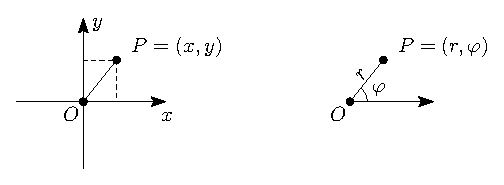
\includegraphics[width=0.45\textwidth]{CDGL1_7.eps}
	\caption{Задание системы координат.}
	\label{1_7}
\end{figure}
Введём полярные координаты, тогда:
$$
	P = (r,\varphi) \Rightarrow f(r,\varphi) = r
$$
Заметим, что если буквально подходить к обозначению, то было бы: $f(r,\varphi) = \sqrt{r^2 + \varphi^2}$, при этом очевидно, что формулы выше - верны. В геометрии функция определяется не только символом $f$, но ещё и символами, которые стоят в виде аргументов.

У нас задана евклидова плоскость и функция отображающая её в $\MR$. А что такое декартовые координаты $(x,y)$? Что значит, что мы их ввели? Это означает, что по двум числам $(x,y)$ мы можем построить точку в нашей евклидовой плоскости, тогда у нас появляется отображение:
$$
	\Phi \colon \MR^2 \to \MBE^2, \quad \Phi(x,y) = P
$$
Аналогично, мы можем построить отображение из полярной системы координат:
$$
	\Psi \colon \MR^2 \to \MBE^2, \quad \Psi(r,\varphi) = P
$$
Следовательно, никакого $f(x,y)$ или $f(r,\varphi)$ у нас нет, формально говоря, поскольку в $f$ мы можем подставлять только точки из $\MBE^2$. Таким образом, что у нас на самом деле есть:
$$
	f \circ \Phi (x,y) = \sqrt{x^2 + y^2}, \quad f \circ \Psi (r,\varphi) = r
$$
Строго говоря, формулы должны иметь вид выше, но никто так не делает, потому что с этим не очень привычно работать. Для этого говорят, что $f$ в координтах $x,y$ имеет вид: 
$$
	f(x,y) = \sqrt{x^2 + y^2}
$$
Или $f$ в координатах $r,\varphi$ имеет вид:
$$
	f(r,\varphi) = r
$$
\subsection*{Замена координат}
В алгебре и в анализе функции определяются своими символами, тогда как в геометрии они определяются как обозначением самой функцией, так и обозначением её аргументов. Особенно заметно это становится при замене координат. Формула перехода из полярных координат в декартовы:
$$
	x = r\cos{\varphi}, \, y = r\sin{\varphi} \Rightarrow x = x(r,\varphi), \, y = y(r,\varphi)
$$
Тогда мы получим такое странное равенство (поскольку $f$ справа и слева обозначают разные вещи):
$$
	f(x(r,\varphi),y(r,\varphi)) = f(r,\varphi)
$$
где справа имеется в виду функция: $f(r,\varphi) = r$, а слева: $f(x,y) = \sqrt{x^2 + y^2}$, тогда:
$$
	\sqrt{r^2{\cdot}\cos^2{\varphi} + r^2{\cdot}\sin^2{\varphi}} = r
$$
Следовательно, путь нашего отображения будет имеет вид:
$$
	\MR^2\colon (r,\varphi) \xrightarrow{\Psi}\MBE^2 \xrightarrow{\Phi^{-1}} \MR^2 \colon (x,y) \xrightarrow{f\circ \Phi} \MR \Rightarrow f\circ \Phi \circ \Phi^{-1}\circ \Psi = f \circ \id \circ \Psi = f\circ \Psi
$$
В предыдущем примере было так:
$$
	\vec{r}(t) \Rightarrow \vec{r}(\varphi(\tau)) = \vec{r}(\tau)
$$
Здесь у нас есть два разных параметра, описывающих точку на кривой и понимать эти формулы мы будем аналогично замене координаты выше: $\vec{r}(t)$ и $\vec{r}(\tau)$ - разные кривые, которые связаны с помощью замены параметров.

\section*{Кривизна кривой}
Далее мы будем работать с ГРП кривыми в евклидовых пространствах. Есть несколько способов приблизиться к кривизне, а поскольку у нас кривая задана параметрически, то и к кривизне мы подойдем параметрически. Интуитивно, чем более загнута кривая, тем больше кривизна. Как её измерить?
\begin{figure}[H]
	\centering
	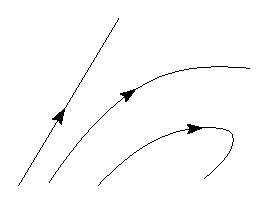
\includegraphics[width=0.25\textwidth]{CDGL1_8.eps}
	\caption{Интуитивное увеличение кривизны кривых.}
	\label{1_8}
\end{figure}
Рисунок может натолкнуть на мысль, что когда мы обычно едем по извилистой дороге, то нас обычно кидает из стороны в сторону, потому что есть центробежная сила. По закону Ньютона:
$$
	\vec{F} = m{\cdot}\vec{a} = m{\cdot}\ddot{\vec{r}}
$$
где $\vec{F}$ - сила, $m$ - масса, $\vec{a}$ - ускорение и $\vec{r}$ - наш вектор-радиус. Равенства верные, поскольку ускорение это вторая производная от нашей координаты. Далее, будем опускать вектор-стрелки. Оказывается, что сила пропорциональна ускорению, если мы едем по более искривленному пути, то нас бросает больше, поэтому эту силу можно принять за меру кривизны кривой. Тем не менее, на тела разной массы действует разная сила, будем брать всегда тествое тело массой $1$: $m = 1$ и с помощью него мерить кривизну. 

Помимо этого, мы знаем, что сила также будет зависеть от скорости: если мы едем на старом автобусе, то прижимать нас будет слегка, но если мы едем на быстрой гоночной машине, то прижимать будет гораздо сильнее $\Rightarrow$ помимо стандартной массы нам необходима некоторая стандартная скорость:
$$
	|\dot{\vec{r}} \, | = 1
$$
Следовательно, мы будем просто смотреть на длину ускорения, тогда кривизна: $k = |\ddot{\vec{r}}|$. Если у нас есть какая-то заданная кривая, то скорость у нас уже есть, что значит скорость равная $1$? Это означает, что нам нужно как-то перепараметризовать нашу кривую: ввести другой параметр, так, чтобы скорость была равна единице. Возможно ли это вообще сделать?

\subsection*{Существование натурального параметра на кривой}

\begin{defn}
	Параметр $s$ на кривой $\vec{r}(s)$ называется \uwave{натуральным}, если $|\dot{\vec{r}} \, | \equiv 1$.
\end{defn}
Пусть у нас задана некоторая кривая $r(t)$ с $t \in [a,b]$.
\begin{figure}[H]
	\centering
	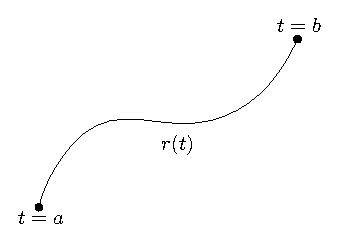
\includegraphics[width=0.25\textwidth]{CDGL1_9.eps}
	\caption{Заданная кривая $r(t)$.}
	\label{1_9}
\end{figure}
Из математического анализа мы знаем, что длина этой кривой определяется по формуле:
$$
	l = \ddint{a}{b}|\dot{r}|dt = \ddint{a}{b}\sqrt{(\dot{x}^1(t))^2 + \dotsc + (\dot{x}^n(t))^2}dt
$$
В каком смысле мы можем взять длину в качестве параметра? Выберем на нашей кривой некоторую точку $r(t_0)$, на ней также задана ориентация. Договоримся, что $\forall t > t_0, \, l(t) > 0$ и $\forall t < t_0, \, l(t) < 0$.
\begin{figure}[H]
	\centering
	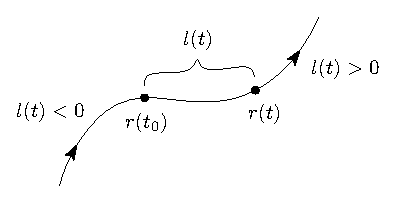
\includegraphics[width=0.3\textwidth]{CDGL1_10.eps}
	\caption{Длина дуги $(r(t_0), r(t))$.}
	\label{1_10}
\end{figure}
Такая договоренность отвечает следующему определению:
$$
	l(t) = \ddint{t_0}{t}|\dot{r}(t)|dt
$$
Рассмотрим тогда производную $l(t)$ (дифференцируем интеграл):
$$
	\dfrac{dl}{dt} = |\dot{r}(t)| > 0
$$
где неравенство верно в силу регулярности кривой. По теореме об обратной функции: $t = t(l)$, тогда мы можем сделать замену параметра:
$$
	r(t(l)) = r(l)
$$
То есть мы \textbf{параметризовали кривую через её длину}. Тем не менее этот процесс не тривиальный: посчитать интеграл - тяжело и найти обратную функцию для которой гарантируется существование - также трудно.
При этом у длины есть нужное нам свойство.

\begin{prop}
	Длина $l$ - натуральный параметр.
\end{prop}
\begin{proof}
	Нам нужно найти длину $\tfrac{dr}{dl}$, если она будет равна $1$, то мы докажем утверждение. По теореме о дифференцировании сложной функции и по теореме об обратной функции:
	$$
		\dfrac{dr}{dl} = \dfrac{dr}{dt}{\cdot}\dfrac{dt}{dl} = \dfrac{dr}{dt}{\cdot}\dfrac{1}{\tfrac{dl}{dt}} = \dfrac{dr}{dt}{\cdot}\dfrac{1}{\left|\tfrac{dr}{dt}\right|} \Rightarrow \left|\dfrac{dr}{dl}\right| = \dfrac{\left|\tfrac{dr}{dt}\right|}{\left|\tfrac{dr}{dt}\right|} = 1
	$$
	где мы воспользовались равенством выше: $\tfrac{dl}{dt} = |\dot{r}(t)|$.
\end{proof}
Таким образом, на любой кривой можно ввести натуральный параметр. Единственен ли этот параметр?

\subsection*{Единственность натурального параметра на кривой}

\begin{prop}
	Любой натуральный параметр (с той же ориентацией) является длиной с точностью до сдвига.
\end{prop}
\begin{proof}
	Пусть $s$ - это какой-то натуральный параметр и $l$ - это длина (одна из тех длин, которые определили выше), тогда продифферецнируем длину по этому параметру: 
	$$
		l = \ddint{s_0}{s}\left|\dfrac{dr}{ds}\right|ds \Rightarrow \dfrac{dl}{ds} = \left|\dfrac{dr}{ds}\right| = 1 \Rightarrow l = s + \const
	$$
	Следовательно, любой натуральный параметр это длина плюс какая-то константа.
\end{proof}
\begin{figure}[H]
	\centering
	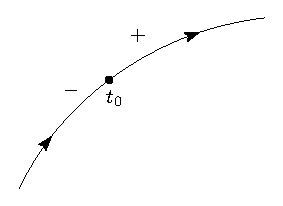
\includegraphics[width=0.2\textwidth]{CDGL1_11.eps}
	\caption{Определение натурального параметра по исходной ориентации.}
	\label{1_11}
\end{figure}
\begin{rem}
	Мы натуральный параметр определяли так, что он имеет ту же ориентацию, что и наш исходный параметр, с помощью которого мы его строили. При желании можно делать наоборот, но если считаем, что ориентация  - та же, то у нас будет просто сдвиг между разными натуральными параметрами относительно длины.
\end{rem}
Также заметим, что если у нас есть две длины связанные с разными базисными точками, то они будут отличатся на сдвиг равный длине между базисными точками. 
\begin{figure}[H]
	\centering
	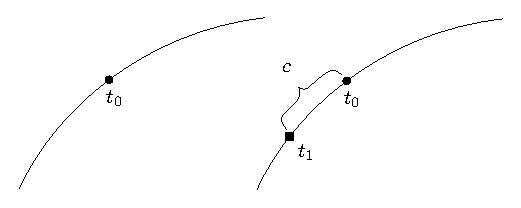
\includegraphics[width=0.4\textwidth]{CDGL1_12.eps}
	\caption{Разные базисные точки.}
	\label{1_12}
\end{figure}
Например, если длина сдвига между $t_1$ и $t_0$ - $c$, первая длина - $l$ от $t_0$, вторая - $\wte{l}$ от $t_1$, то тогда:
$$
	\wte{l} = c + l
$$
Следовательно, если у нас кривая бесконечна в обе стороны (определена в интервале от $-\infty$ до $+\infty$), то константу всегда можно проинтерпретировать как выбор другой базисной точки $\Rightarrow$ любой натуральный параметр является длиной для какого-то выбора начальной точки.

\subsection*{Кривизна натурального параметра}
\begin{defn}
	Для кривой в натуральной параметризации \uwave{кривизной} в некоторой точке, отвечающей параметру $s$, называется длина ускорения:
	$$
		k(s) = \left| \dfrac{d^2 \vec{r}}{ds^2}(s) \right|
	$$
\end{defn}

\begin{defn}
	Для кривой в произвольной параметризации \uwave{кривизной} в некоторой точке, отвечающей параметру $s$ называется длина ускорения перепараметризованной кривой в натуральной параметризации.
\end{defn}

\begin{exrc}
	Если кривая в $\MR^2$ или в $\MR^3$, то при произвольном параметре нужно взять длину векторного произведения скорости и ускорения и разделить её на длину вектора скорости в $3$-ей степени:
	$$
		k(t) = \dfrac{\left|[\dot{r},\ddot{r}]\right|}{|\dot{r}|^3}
	$$
\end{exrc}
\newpage

\section*{Плоские кривые}



\end{document}